\documentclass[12pt]{szablon}

\usepackage[utf8]{inputenc}   %jezyk polski
\usepackage{polski}             %jezyk polski

\usepackage[centertags]{amsmath}
\usepackage{amsfonts}
\usepackage{amssymb}
\usepackage{amsthm}
\usepackage{newlfont}
\usepackage{graphicx}
\usepackage{wrapfig}
\usepackage{color}
%\usepackage{indentfirst}
\brokenpenalty=10000 %nie dieli wyrazów pomiędzy stronami
%\linespread{1.3} %odstęp pomiędzy wierszami 1.5 linii
\sloppy %zakaz wydłużania lini (gdy nie może złożyć)
\clubpenalty=10000 %to kara za sierotki
\widowpenalty=10000
%	\renewcommand{\baselinestretch}{1.3}
\linespread{1.3} %interlinia
\usepackage{lipsum}%przykłaDOWY tekst
% -- otoczenia


\newtheorem{tw}{{\sf Twierdzenie}}[chapter]  %definicja otoczenia Twierdzenie
\newtheorem{lem}[tw]{{\sf Lemat}}     %definicja otoczenia Lemat
\newtheorem{wn}[tw]{{\sf Wniosek}}     %definicja otoczenia Wniosek
\newtheorem{wl}[tw]{\sf Własność} %definicja otoczenia Właasność

\theoremstyle{definition}
\newtheorem{deff}[tw]{{\sf Definicja}}  %definicja otoczenia Definicja
\newtheorem{pr}[tw]{{\sf Problem}}     %definicja otoczenia Problem
\newtheorem{przykl}[tw]{{\sf Przykład}} %definicja otoczenia Przykład
\newtheorem{uw}[tw]{{\sf Uwaga}}       %definicja otoczenia Uwaga
\renewcommand{\theequation}{{\thechapter}.\arabic{equation}} %sposób numeracji wzorów


% -- układ strony

\textwidth 15.5cm
\textheight 23cm
\topmargin -1.cm
\setlength{\oddsidemargin}{1cm}
\setlength{\evensidemargin}{1cm}

% -- głębokość numeracji w spisie treści

\setcounter{tocdepth}{2} \setcounter{secnumdepth}{2}

%

\def\thefootnote{\arabic{footnote})}

%----- czcionka

\renewcommand{\familydefault}{\sfdefault} % for calibri

%\renewcommand{\familydefault}{\rmdefault} % for times

% -- dokument

\begin{document}

%-- Strona tytułowa -----




\begin{titlepage}
\begin{tabular}{@{}cc@{}}
\begin{tabular}{@{}l@{}@{}}
\tabularnewline[2em]
 \hspace{-1.5cm} \large{ \  \textsf{\bf UNIWERSYTET RZESZOWSKI}} \tabularnewline[0.1cm]
 \hspace{-1.5cm} \large{ \  \textsf{\bf Kolegium Nauk Przyrodniczych}} \tabularnewline[0.1cm]
\end{tabular} &
\begin{tabular}{@{}c@{}}
	\hspace{6cm}
\includegraphics[width=8em]{logoUR2.jpg}
\end{tabular} 
\end{tabular} 

\vspace{3cm}
\begin{center}
{\Large\textsf{Imię i Nazwisko studenta}}   \\    %wpisać imię i nazwisko
{\large\textsf{nr albumu: XXXXXXXXX   }}\\       %wpisac numer albumu
{\large\textsf{Kierunek: Informatyka}}\\       
\vspace{2cm}
{\LARGE\bf\textsf{Tytuł (temat) pracy dyplomowej }}  \\ \vspace{3ex}
{\LARGE\bf\textsf{Tytuł Tytuł Tytuł Tytuł Tytuł }} %wpisać tytuł pracy
\end{center}
\vspace{1.5cm}

\hspace{6cm}
\begin{minipage}[l]{18em}
	{\large\textsf{Praca licencjacka/magisterska}}
\end{minipage}

\vspace{1.5cm}

\hspace{7cm}
\begin{minipage}[l]{18em}
{\large\textsf{Praca wykonana pod kierunkiem}\\     %właściwe zostawić
\textsf{imię i nazwisko promotora}}                  %wpisać promotora pracy
\end{minipage}

\vspace{3cm}

\begin{center}
{\large\textsf{ Rzeszów, 2022}} %wpisać prawidłowy rok
\end{center}
\end{titlepage}

\newpage

%
%--- Wersja polska------------------

\begin{titlepage}
\begin{tabular}{@{}cc@{}}
\begin{tabular}{@{}c@{}}
  \hskip -1.5cm  
\includegraphics[width=30mm]{logoUR2.jpg}
\end{tabular} &
\begin{tabular}{@{}l@{}@{}}
\tabularnewline[2em]
 %\LARGE 
  \  {\fontsize{40}{48} \textsf{Uniwersytet Rzeszowski} } \tabularnewline[0.1cm]
 %\LARGE FACSO \tabularnewline[0.1cm]
% \LARGE \ \textsf{Kolegium Nauk Przyrodniczych} \tabularnewline[0.1cm]
\end{tabular} \tabularnewline[3cm]
& \large\textsf{Kierunek: Matematyka}\tabularnewline[.5 \baselineskip]
& {\large\textsf{Studia: stacjonarne/ niestacjonarne}} \tabularnewline[3cm]% wybrać
& \tabularnewline[\baselineskip]
%\tabularnewline[0.4cm]
\end{tabular} 
%\multicolumn{2}{c} 
\vspace{-1cm}
\begin{center}
{\LARGE\textsf{ Autor}}   \\    %wpisać imię i nazwisko
%\tabularnewline[0.1cm]
%\multicolumn{2}{c} 
{\large\textsf{nr albumu:}}\\       %wpisac numer albumu
%\tabularnewline[2cm]
%\multicolumn{2}{c} 
\vspace{2cm}
{\LARGE\bf\textsf{Tytuł Tytuł Tytuł Tytuł Tytuł }}  \\ \vspace{3ex}
{\LARGE\bf\textsf{Tytuł Tytuł Tytuł Tytuł Tytuł }} %wpisać tytuł pracy
\end{center}

\vspace{3cm}

\hspace{7cm}
\begin{minipage}[l]{18em}
{\large\textsf{Praca licencjacka/magisterska}\\     %właściwe zostawić
\textsf{wykonana w Instytucie Matematyki \\
pod kierunkiem} \\
\textsf{imię i nazwisko promotora}      %wpisać promotora pracy
}
\end{minipage}

\vspace{3cm}

\begin{center}
{\large\textsf{ Rzeszów 2019}} %wpisać prawidłowy rok
\end{center}
\end{titlepage}
%---------------Wersja angielska-------------------------------------------


\begin{titlepage}
\begin{tabular}{@{}cc@{}}
\begin{tabular}{@{}c@{}}
  \hskip -1.5cm 
\includegraphics[width=30mm]{logoUR2.jpg}
\end{tabular} &
\begin{tabular}{@{}l@{}@{}}
\tabularnewline[2em]
% \LARGE \ 
  \  {\fontsize{40}{48} \textsf{University of Rzeszów} } \tabularnewline[0.1cm]
 %\LARGE FACSO \tabularnewline[0.1cm]
% \LARGE \ \ \textsf{College of Natural Sciences} \tabularnewline[0.1cm]
\end{tabular} \tabularnewline[3cm]
& \large\textsf{The field of study: Mathematics}\tabularnewline[.5\baselineskip]
& \large\textsf{Types of studies: full-time/ part-time} \tabularnewline[3cm]% wybrać
& \tabularnewline[\baselineskip]
\end{tabular} 
\vspace{-1cm}
\begin{center}
{\LARGE\textsf{ Author}}  \\     %wpisać imię i nazwisko
%\tabularnewline[0.1cm]
%\multicolumn{2}{c} 
{\large\textsf{nr albumu}} \\      %wpisac numer albumu
%\tabularnewline[2cm]
%\multicolumn{2}{c} 
\vspace{2cm}
{\LARGE\bf\textsf{Title Title Title Title Title Title Title }}\\  \vspace{3ex}
{\LARGE\bf\textsf{ Title Title Title  Title Title 
Title Title Title }}       %wpisać tytuł pracy
\end{center}


\vspace{3cm}

\hspace{5cm}
\begin{minipage}[l]{21em}
{\large\textsf{Type of the thesis: Msc./Bsc.}\\    %właściwe zostawić
\textsf{The thesis written \\
in the Institute of Mathematics\\
under the supervision of} \\
\textsf{imię i nazwisko promotora}}       %wpisać promotora pracy
\end{minipage}

\vspace{2cm}

\begin{center}
{\large\textsf{ Rzeszów 2019}} %wpisać prawidłowy rok
\end{center}
\end{titlepage}

%--------------------------------------
\newpage




% -- spis treści

\setcounter{page}{0} \tableofcontents\thispagestyle{empty}


% -- zawartość pracy

\chapter*{WSTĘP}
\addcontentsline{toc}{chapter}{\protect\hspace{0.45cm} WSTĘP}

{\markboth{}{}
\setlength{\parskip}{1.2ex plus 0.5ex minus 0.2ex}
\baselineskip 0.6cm

Tekst wstępu \\

\lipsum[1-2] % usunąć linię

}


\chapter{TYTUŁ ROZDZIAŁU PIERWSZEGO}

{%\markboth{}{}
%\setlength{\parskip}{1.2ex plus 0.5ex minus 0.2ex}
%\baselineskip 0.6cm

%\lipsum % usunąć linię
\section{Numerowanie}
\textit{To czcionka       pochylona}. \\
Tekst piszemy standardowo nie przejmując się ilością spacji Tekst pierwszego rozdziału  aa
ma spełniać dwa warunki:
\begin{itemize}
    \item warunek 1 hgi;ghasioga kjabsgkjasb sakgjbas;kjbas askgbasd;kgasbgb;a sdvafd afd ad fb afdb daf b adfb afd bad fb adf
    \item war2
\end{itemize}
\subsection{nowe}
\begin{itemize}
	\item[$\star$] tuygfasgl
	\item[$\star$] ksdbvalskval
\end{itemize}
\begin{enumerate}
	\item warunek 2
	\item warynenckjd
\end{enumerate}

\section[skrót]{Wzory matematyczne}
W tekście wzory piszemy następująco $wzor$ i już. $y=x_{11}^2$ $x_{132425}^{ads}$

Wzór wyeksponowany

nienumerowany
$$
F(x)=\sqrt{x_1^3}
$$

numerowany
\begin{equation}
	\label{eq: wczesniej}
	x^2
\end{equation}

\begin{equation}
	\label{eq:cos} %etykieta wzoru
	F(x)=\frac{x_1^2}{\sqrt{2x-4}}
\end{equation}
We wzorze \eqref{eq:cos} należy coś zrobić

Granice wyrażeń
$$
\lim\limits_{x\rightarrow \infty} \frac{x-3}{x^2+5}
$$

$f'(x), f''(x), f'''(x),\ \ \  f^{(iv)}(x)$

$$
\sum_{i=1}^{\infty} \frac{i}{i+1}
$$

$$
\int f(x) dx ,\ \ \int_{1}^{3} f(x) dx \ \ \ \int\limits_5^6 f(x) dx \ \ 
\iint f(x) \iiint\limits_{1}^3
$$

$x\in \mathbb{R, N, Z, C}$ 

$x\notin R$

Kroje pisma standardowy, \textit{kursywa}, \textbf{wytłuszczenie}, \underline{podkreślenie} \textcolor{green}{tekst kolorowy}

Kroje pisma matematycznego $standard\ to\ kursywa $, $\mathrm{tekst}$, $\mathbf{pogrubiony}$  $\mathcal{kaligrafia}$

$$
x>0, x<0, x\geq 0, x\le 0, x\leqq 7
$$

Równania wielowierszowe
\begin{equation*}
	f(x)=\left(\frac{\frac{1}{x+3}}{x-4}\right)
\end{equation*}
%http://www.latex-kurs.x25.pl/paper/wyrazenia_matematyczne
$$
\left[
\begin{array}{cccc}
	a_{11} & a_{22} & \cdots & a_{33} \\
	a_{21} & a_{22} & \ddots & a_{23} \\
	a_{31} & a_{32} & \ldots & \vdots
\end{array}
\right]_{n\times n}
$$

\begin{equation*}
	f(x)=\left\{ \begin{array}{cl}
		x, & \text{gdy } x\geq 0,\\
		-x, & x<0.			
	\end{array}
	\right.
\end{equation*}

\begin{eqnarray}
	f(x) & = & \cos x \\
	f'(x) & = & -\sin x \\
	\int_{0}^{x} f(y)dy &
	= & \sin x
\end{eqnarray}


\begin{eqnarray}
	f(x) & = & \cos x  sdxse ef e f ef e fe f e fe f+ fw- fe + \nonumber\\
	 &  & -\sin x 
\end{eqnarray}

\begin{multline}
	a+b+c+d+e+f+g+h+i+j+k+\\
	l+m+n+o+p+q+r+s+t+w+x+y+z\\
	l+m+n+o+p+q+r+s+t+w+x+y+z
\end{multline}



Przykład tabeli
\begin{table}
\label{tab:numer}
\begin{center}
\begin{tabular}{ |c |c| l| }
\hline
 cell1 & cell2 & cell3 \\ 
 \hline\hline
 cell4 & c5 & ce \\ 
 \hline
 cell7 & cell8 & cell9  \\ 
 \hline
\end{tabular}
\end{center}
\caption{Podpis tabeli}
\end{table}

Przykład rysunku
\begin{figure}%[!b]
	\centering \includegraphics[width=0.9\textwidth]{img/Ti-xy3-3x2_kopia.jpg}
	\caption{Logo UR.}
\label{figure_1a}
\end{figure}

\begin{figure}%[!h]
	\centering 
	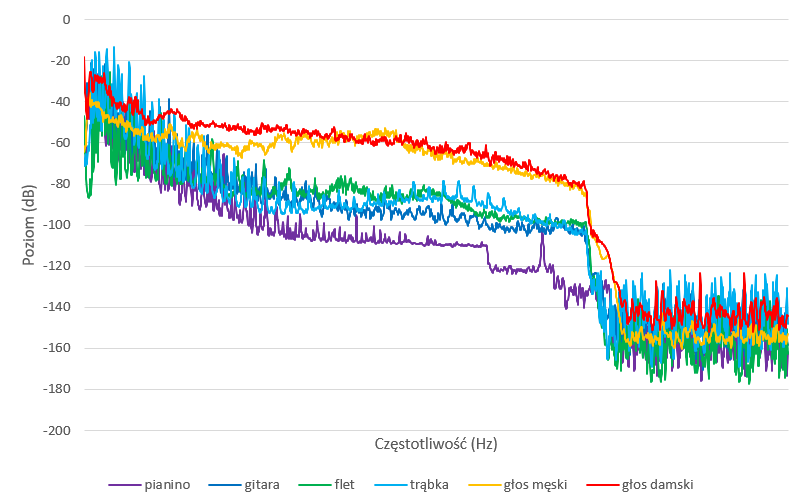
\includegraphics[trim= 0 0 150 150, clip, angle=45, width=0.9\textwidth]{wykres.png}
	\caption{Dziwny wykres}
\label{figure_1b}
\end{figure}

To jest {\textbf{grube}} a to jest \textit{pochyłe}


}

\chapter{TYTUŁ ROZDZIAŁU  DRUGIEGO}

{\markboth{}{}
\setlength{\parskip}{1.2ex plus 0.5ex minus 0.2ex}
\baselineskip 0.6cm

Tekst drugiego rozdziału\\

\lipsum[1-2] % usunąć linię

}

\chapter{TYTUŁ ROZDZIAŁU  TRZECIEGO}

{\markboth{}{}
\setlength{\parskip}{1.2ex plus 0.5ex minus 0.2ex}
\baselineskip 0.6cm

Tekst trzeciego rozdziału

}

\chapter*{ZAKOŃCZENIE}
\addcontentsline{toc}{chapter}{\protect\hspace{0.45cm} ZAKOŃCZENIE}

{\markboth{}{}
\setlength{\parskip}{1.2ex plus 0.5ex minus 0.2ex}
\baselineskip 0.6cm

Tekst zakończenia

}


\newpage

\def\bibname{\centerline{{\LARGE{LITERATURA}}}}

\begin {thebibliography}{99}\markboth{LITERATURA}{}
\addcontentsline{toc}{chapter}{\protect\hspace{0.45cm} LITERATURA}



\bibitem{BSU}
Y.M. Berezansky, Z.G. Sheftel, G.F. Us, {\it Functional Analysis},
Birkh{\"a}user Verlag, Basel - Boston - Berlin, 1996.

\bibitem{Fish}
B. Fisher, {\it The product of distributions}, Quart. J. Math. Oxford {\bf
22} (1971), 291--298.

\bibitem{Lo}
S. Łojasiewicz, {\it Wstęp do teorii funkcji rzeczywistych}, PWN, Warszawa,
1973.

\bibitem{Ox}
J.C. Oxtoby, {\it Measure and Category}, Springer--Verlag, New York -
Heidelberg - Berlin, 1971.

\end{thebibliography}

\chapter*{STRESZCZENIE}
\addcontentsline{toc}{chapter}{\protect\hspace{0.45cm} STRESZCZENIE}

{\markboth{}{}
\setlength{\parskip}{1.2ex plus 0.5ex minus 0.2ex}
\baselineskip 0.6cm

\noindent {\bf Tytuł pracy w języku polskim:}\\

\noindent {\bf Tytuł pracy w języku angielskim:}\\


\noindent {\bf Streszczenie:}\\
\indent Tekst streszczenia  

\lipsum[1-2]  % tę linię usunąć

}

\end{document}
